\subsection{Схемы из функциональных элементов и простейшие алгоритмы их синтеза. Оценка сложности схем, получаемых по методу Шеннона.}

\textbf{Орграф} -- это ориентированный граф.

Вершины орграфа, в которые не входит ни одной дуги, называются \textbf{истоками}.

Орграф называется \textbf{ациклическим}, если в нем нет ориентированных циклов.

Систему Б = {$g_1$, $g_2$, ..., $g_m$}, где все $g_i$ — функции алгебры логики, будем называть \textbf{базисом функциональных элементов}.

Орграф называется \textbf{упорядоченным}, если для каждой вершины $v_i$, в которую входит $k_i$ дуг, задан порядок $e_1$, $e_2$, ..., $e_{k_i}$ этих дуг.

\bigbreak

\textbf{Схемой из функциональных элементов} в базисе Б называется ациклический упорядоченный орграф, в котором:
\begin{itemize}
    \item каждому истоку приписана некоторая переменная, причем разным истокам приписаны разные переменные (истоки при этом называются входами схемы, а приписанные им переменные — входными переменными);
    \item каждой вершине, в которую входят k $\geq$ 1 дуг, приписана функция из базиса Б, зависящая от k переменных(вершина с приписанной функцией при этом называется \textbf{функциональным элементом}); 
    \item некоторые вершины выделены как \textbf{выходы}. 
\end{itemize}

\textbf{Сложностью} схемы из функциональных элементов называется число функциональных элементов в схеме (число внутренних вершин).

Пример:

\textbf{Полусумматор} Пусть $v$ и $v_1$ — выходы на рисунке, $f_v$ = x$\wedge$y $\wedge$ (x $\vee$ y)= x + y ; $f_{v_1}$ = x$\wedge$y . Сложность (число элементов) полусумматора равна 4.

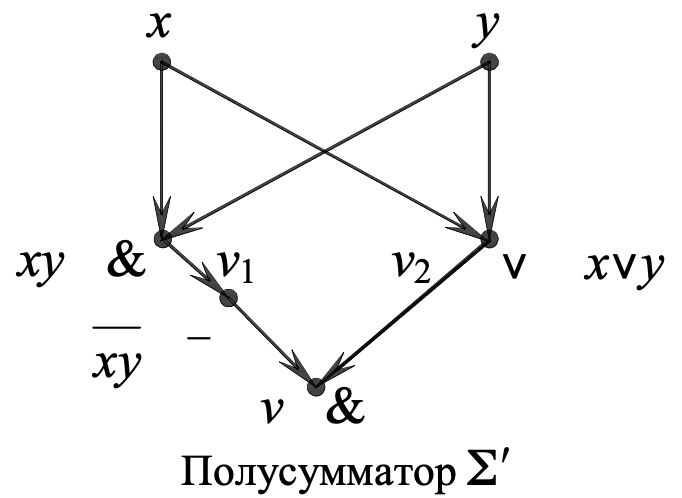
\includegraphics[width=0.5\columnwidth]{pics/pol_sum.png}

% \textbf{Сумматором $S_n$} порядка n называется схема с 2n входами $x_1$, $x_2$, ..., $x_n$, $y_1$, $y_2$, ..., $y_n$ и n + 1 выходом $z_0$, $z_1$, $z_2$, ..., $z_n$ такая, что |$\widetilde{z}$| = |$S_n$ ($\widetilde{x}$,$\widetilde{y}$)| = |$\widetilde{x}$| + |$\widetilde{y}$|.

% \textbf{Теорема} Существует схемный сумматор порядка n в базисе \{$\wedge$, $\vee$, $\bar{}$ \} с числом элементов 9n – 5.

% 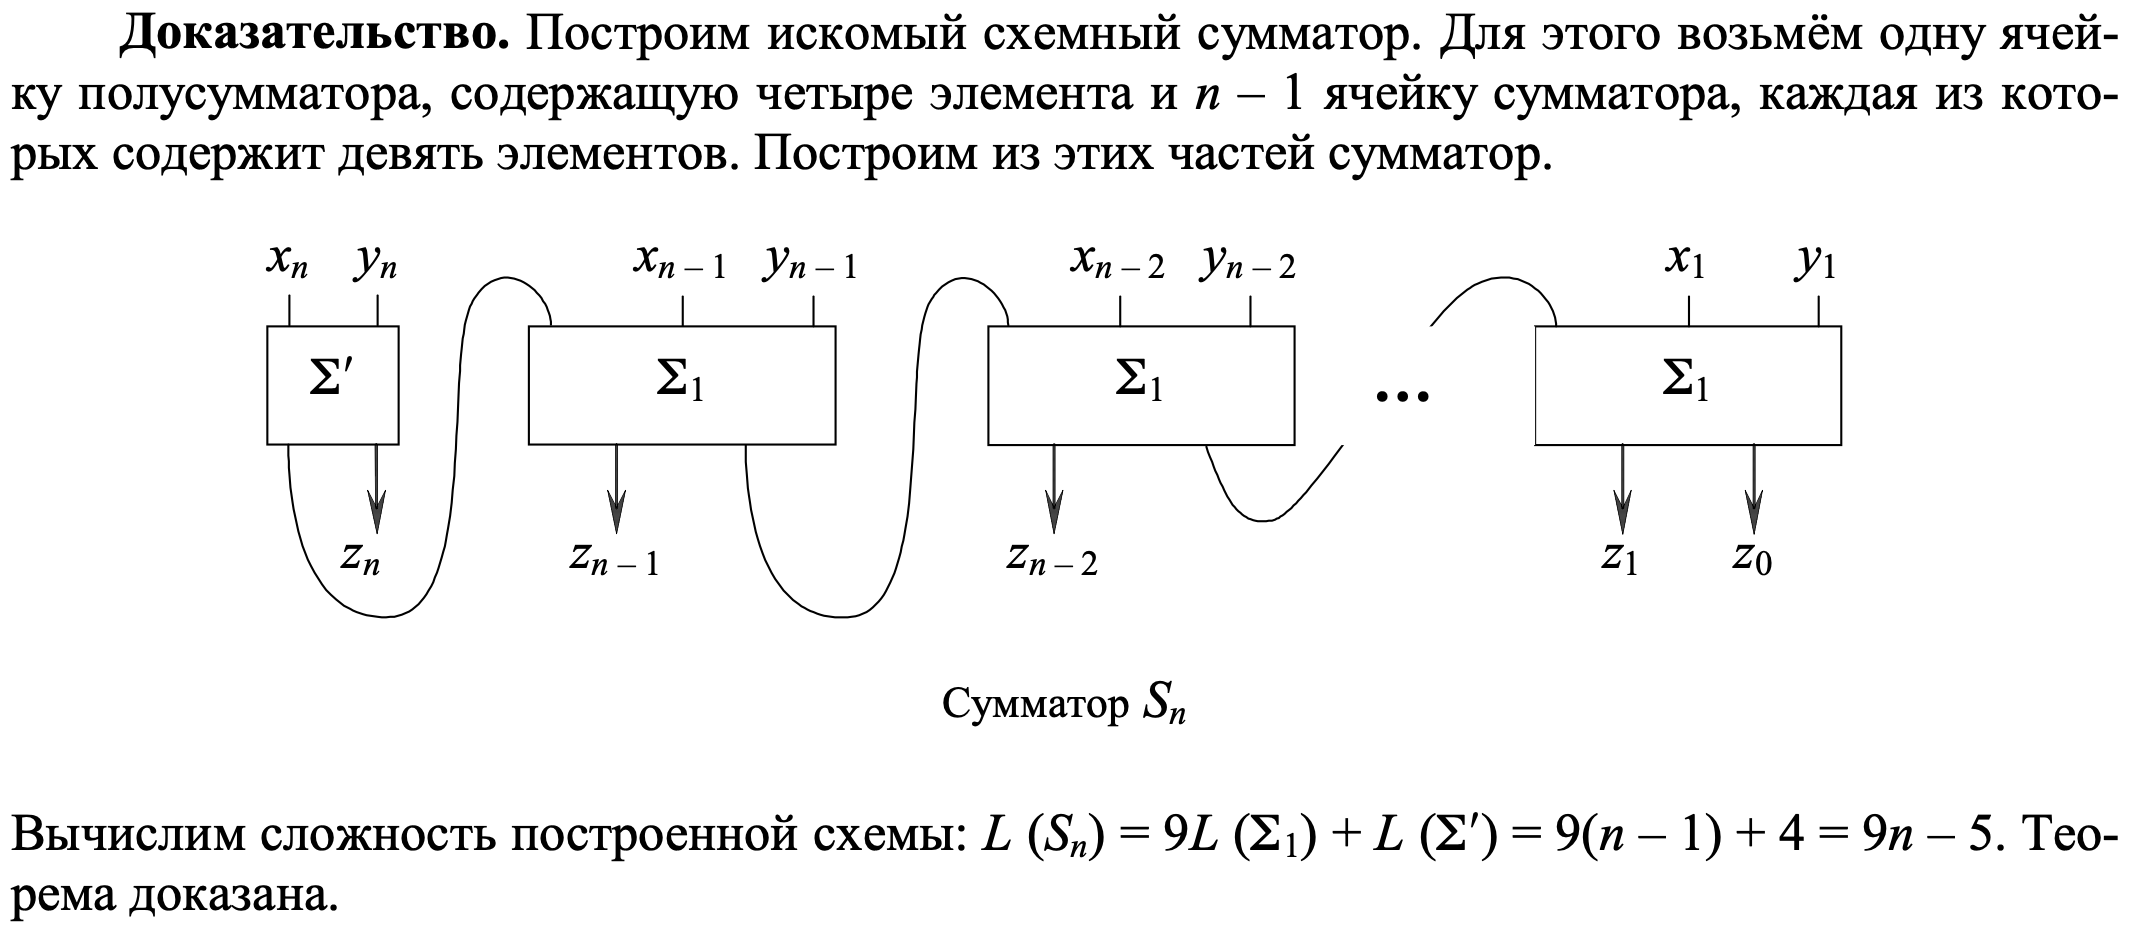
\includegraphics[width=\columnwidth]{pics/sum.png}

% \textbf{Вычитателем $W_n$} порядка n называется схема с 2n входами $x_1$, $x_2$, ..., $x_n$,
% $y_1$, $y_2$, ..., $y_n$ и n выходами $z_1$, $z_2$, ..., $z_n$ такая, что при |x| $\geq$ |y|, |$\widetilde{z}$| = |W ($\widetilde{x}$,$\widetilde{y}$)| = |$\widetilde{x}$| - |$\widetilde{y}$|.

% \textbf{Теорема} Существует схемный вычитатель порядка n в базисе \{$\wedge$, $\vee$, $\bar{}$ \} с числом элементов 9n – 5.

% 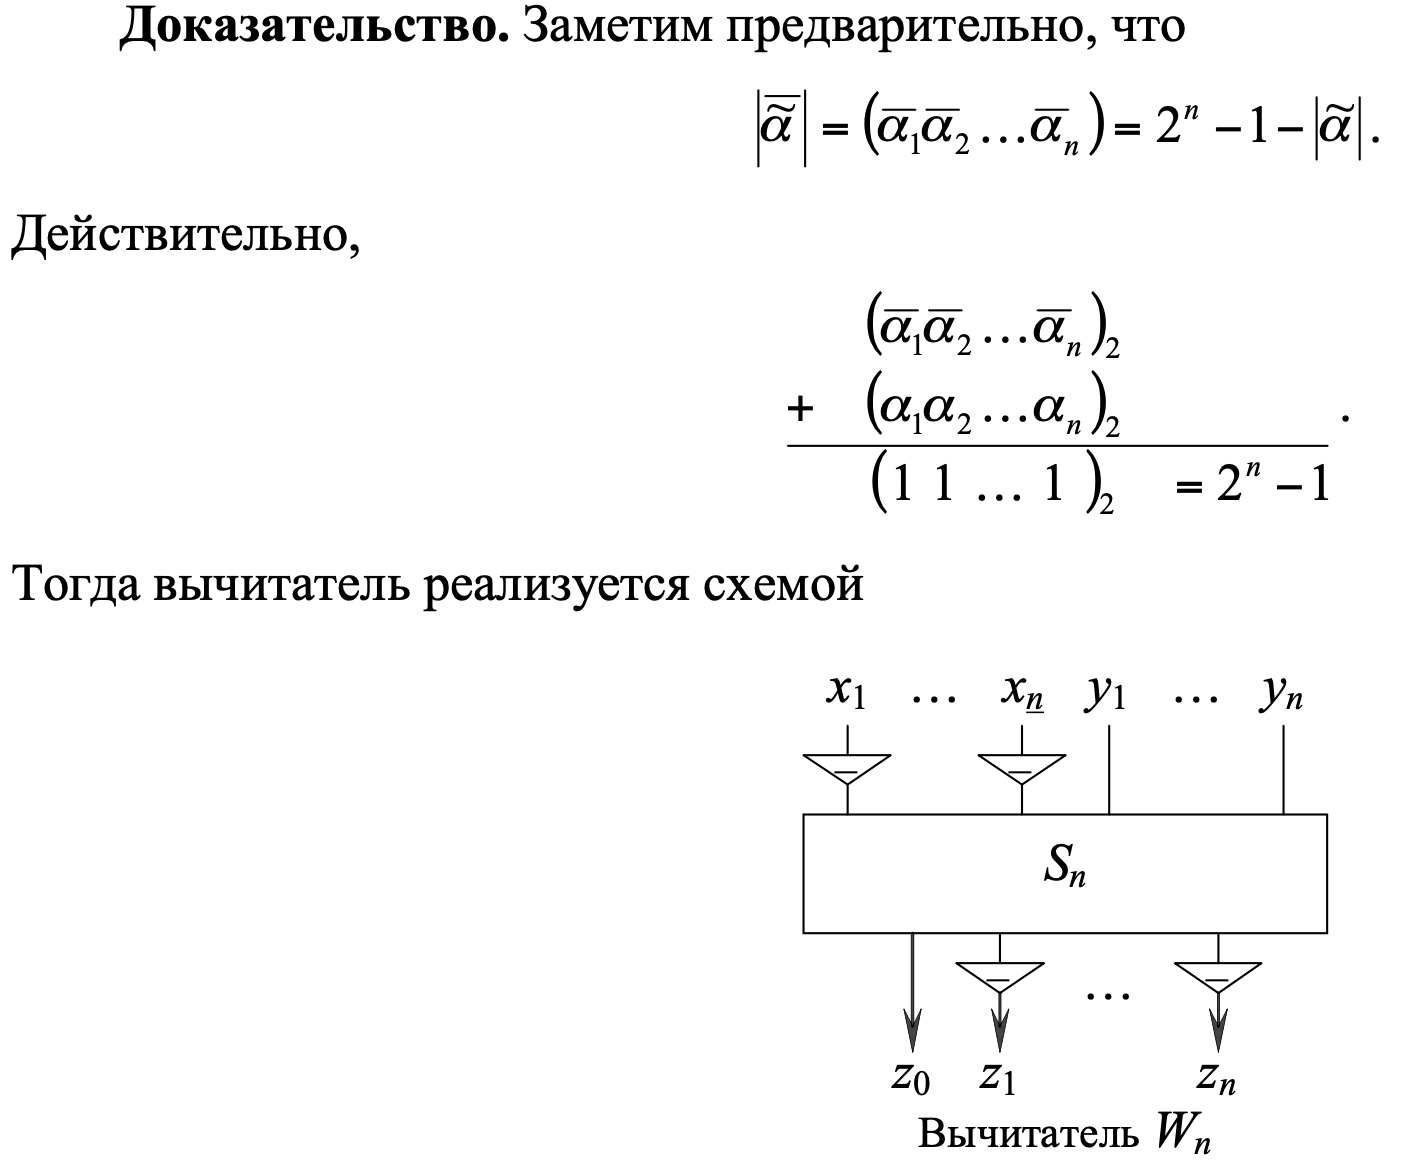
\includegraphics[width=\columnwidth]{pics/wich.png}

% |$W_n$ ($\widetilde{x}$,$\widetilde{y}$)| = |$\widetilde{x}$| - |$\widetilde{y}$| = $2_n$ - 1 - (($2_n$ - 1 - |$\widetilde{x}$|) + |$\widetilde{y}$|)
% и его можно построить, используя 2n отрицаний и 1 сумматор порядка n. При этом L ($W_n$) = 2n + L ($S_n$) = 2n + (9n – 5) = 11n – 5. Поскольку $\widetilde{x}$ $\geq$ $\widetilde{y}$, то ($2_n$ - 1 - |$\widetilde{x}$|) + |$\widetilde{y}$| $\leq$ $2_n$ - 1, и выход вычитателя определен. Теорема доказана.

% \bigbreak

% \textbf{Метод Шеннона.}
    
% Выбираем параметр $q$, $1 \leqslant q \leqslant n$.

% Используется \textbf{разложение Шеннона}:
% $$ f(\underbrace{x_1,\dots,x_q}_{x'},\underbrace{x_{q+1},\dots,x_n}_{x''}) = $$
% $$ = \displaystyle\bigvee_{\sigma''=(\sigma_{q+1},\dots,\sigma_n)} x_{q+1}^{\sigma_{q+1}}\cdots x_n^{\sigma_n}\cdot f_{\sigma''}(x_1,\dots,x_q,\sigma_{q+1},\dots,\sigma_n)$$

% Для любой ФАЛ $f \in P_2(n)$ строим СФЭ $\Sigma_f$ как суперпозицию $\Sigma''(\Sigma')$, где $\Sigma''$ --- мультиплексор, $\Sigma'$ --- универсальный многополюсник.

% 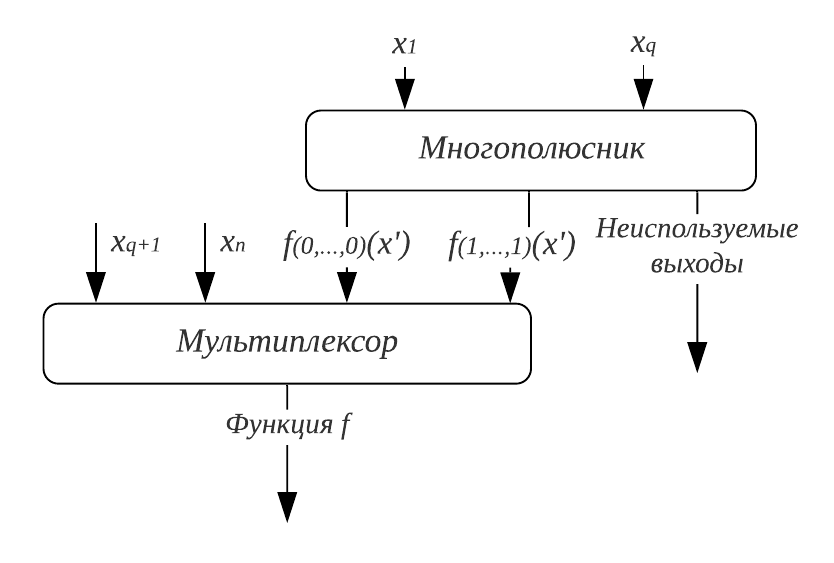
\includegraphics[width=\columnwidth]{pics/osn27_oki.png}
% Схема для $\Sigma_f = \Sigma''(\Sigma')$


% Сложность многополюсника от $q$ переменных: $L(\Sigma') \leqslant 2^{2^q} - q $ (следует из леммы)

% Сложность мультиплексора от $n-q$ переменных: $L(\Sigma'') \leqslant 2^{n - q + 2} - 3$

% Полагая $q = \lfloor \log_2(n - 2\log_2 n) \rfloor$ получаем в результате преобразований: 
% $$ L(\Sigma_f) \leqslant 2^{2^q} + 4\cdot 2^{n - q} \leqslant \frac{8 \cdot 2^n}{n - 2\log n} + O(\frac{2^n}{n^2}) $$

% \textbf{Таким образом, верна оценка сложности СФЭ: }$L^C(n) \lesssim 8 \cdot \frac{2^n}{n}$

\bigbreak
\textbf{Важные ФАЛ и системы ФАЛ:}
\begin{itemize}
    \item Мультиплексорная ФАЛ $\mu_n$ порядка $n$
    $$ \mu(\displaystyle\underbrace{x_1,\dots,x_n}_{\text{адресные}},\displaystyle\underbrace{y_0,\dots,y_{2^n-1}}_{\text{информационные}}) = \displaystyle\bigvee_{\alpha=(\alpha_1,\dots,\alpha_n)} x_1^{\alpha_1} \dots x_n^{\alpha_n} y_{\nu(\alpha)},$$
    где $\nu(\alpha)$ -- перевод двоичного числа $\alpha$ в десятичное.
    
    Реализуется мультиплексором.
    \item Универсальная система $\vec{P_2}(n)$ порядка $n$ --- содержит все ФАЛ от $n$ переменных. Реализуется универсальным многополюсником.
\end{itemize}


\bigbreak
\textbf{Лемма.} Для каждого натурального $n$ существует СФЭ над базисом $B$ $U_n \in U_B^C$(множество всех схем на базисом $B$), которая реализует систему ФАЛ $\vec{P_2}(n)$ и сложность которой равна $2^{2^n} - n$.
    
\begin{proof}
В силу полноты базиса в $U_B^C$ существует система СФЭ $\Sigma$ от БП $x_1,\dots,x_n$, реализующая систему ФАЛ $\vec{P_2}(n)$. Искомая СФЭ $U_n$ является строго приведённой СФЭ, которая эквивалентна $\Sigma$ и получается из неё в результате операций присоединения эквивалентных вершин и удаления висячих вершин. Действительно, из построения следует, что число всех вершин СФЭ $U_n$, включая $n$ её входов, равно $2^{2^n}$ и поэтому $L(U_n) = 2^{2^n} - n$ (вычитаем $n$ входов, которые автоматически реализуют функции $x_1,\dots,x_n$).
\end{proof}

\textbf{Следствие.} $L_B^C(\vec{P_2}(n)) \leqslant 2^{2^n} - n$.

\bigbreak
Базис $B_0 = \{\&, \vee, \neg\}$

\bigbreak
\textbf{Определения сложности.}
    
\textbf{Сложность ФАЛ f}: $L_B(f) = \displaystyle \min_{\substack{\text{СФЭ}~\Sigma \in U_B^C \\ \text{реализующие }f}} L(\Sigma)$

\textbf{Функция Шеннона}: $L_B(n) = \displaystyle \max_{f \in P_2(n)} L_B(f)$
    
\bigbreak
\textbf{Синтез по совершенной ДНФ} 
    
Совершенная ДНФ $f(x_1,\dots,x_n) = \displaystyle\bigvee_{\sigma \in N_f} x_1^{\sigma_1} \&\dots\&x_n^{\sigma_n}$, где $N_f$ --- все наборы $\sigma$, на которых $f(\sigma) = 1$.

Совершенная ДНФ --- формула в $B_0$, значит существует СФЭ $\Sigma_f$ над базисом $B_0$, которая реализует $f$. 

Тогда 
$L(\Sigma_f) \leqslant \underbrace{2^n}_{1}(\underbrace{n - 1}_{2} + \underbrace{n}_{3} ) + \underbrace{2^n - 1}_{4}$,
где 1 --- верхняя оценка $|N_f |$, т.е. количества дизъюнктов в овершенной ДНФ, 2 --- количество конъюнкций в каждом дизъюнкте, 3 --- верхняя оценка количества отрицаний в дизъюнкте, 4 --- оценка количества дизъюнкций между дизъюнктами. СФЭ --- частный случай квазидеревьев, которые эквивалентны формулам, поэтому  $L^C(n) \leqslant L^{\Phi}(n)$
Так получаем верхнюю оценку функции Шеннона: $L^C(n) \leqslant L(\Sigma_f) \leqslant n \cdot 2^{n+1}$.

\bigbreak    
\textbf{Метод Шеннона.}
    
Выбираем параметр $q$, $1 \leqslant q \leqslant n$.

Используется \textbf{разложение Шеннона}:

$f(\underbrace{x_1,\dots,x_q}_{x'},\underbrace{x_{q+1},\dots,x_n}_{x''}) = $ \\
$= \displaystyle\bigvee_{\sigma''=(\sigma_{q+1},\dots,\sigma_n)} x_{q+1}^{\sigma_{q+1}}\cdots x_n^{\sigma_n}\cdot f_{\sigma''}(x_1,\dots,x_q,\sigma_{q+1},\dots,\sigma_n)$

Для любой ФАЛ $f \in P_2(n)$ строим СФЭ $\Sigma_f$ как суперпозицию $\Sigma''(\Sigma')$, где $\Sigma''$ --- мультиплексор, $\Sigma'$ --- универсальный многополюсник.

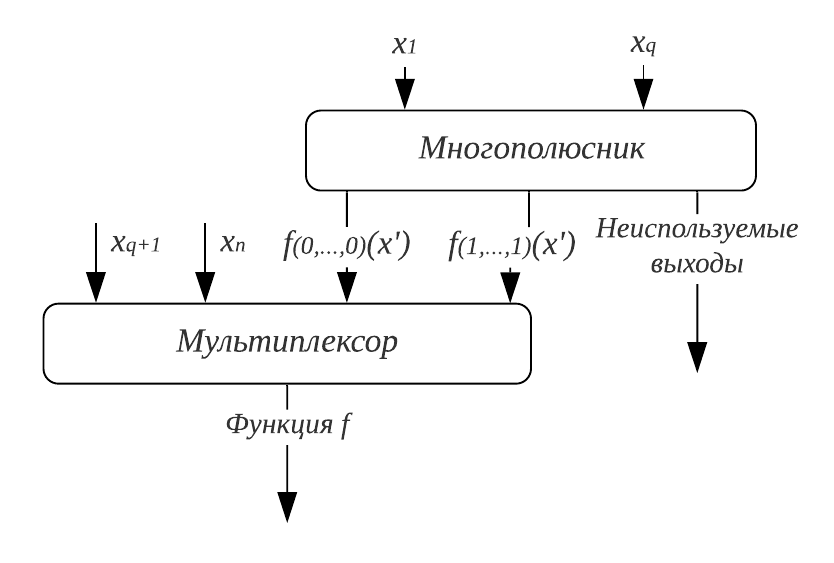
\includegraphics[width=0.9\columnwidth]{pics/osn27_oki.png}

Сложность многополюсника от $q$ переменных: $L(\Sigma') \leqslant 2^{2^q} - q $ (следует из леммы)

Сложность мультиплексора от $n-q$ переменных: $L(\Sigma'') \leqslant 2^{n - q + 2} - 3$

Полагая $q = \lfloor \log_2(n - 2\log_2 n) \rfloor$ получаем в результате преобразований: 
$$ L(\Sigma_f) \leqslant 2^{2^q} + 4\cdot 2^{n - q} \leqslant \frac{8 \cdot 2^n}{n - 2\log n} + O(\frac{2^n}{n^2}) $$

\textbf{Таким образом, верна оценка сложности СФЭ: }$L^C(n) \lesssim 8 \cdot \frac{2^n}{n}$

% -------- source --------
\bigbreak
[\cite[page 69-96]{replace_me}]